\begin{figure}[tbp] 
  \centering
  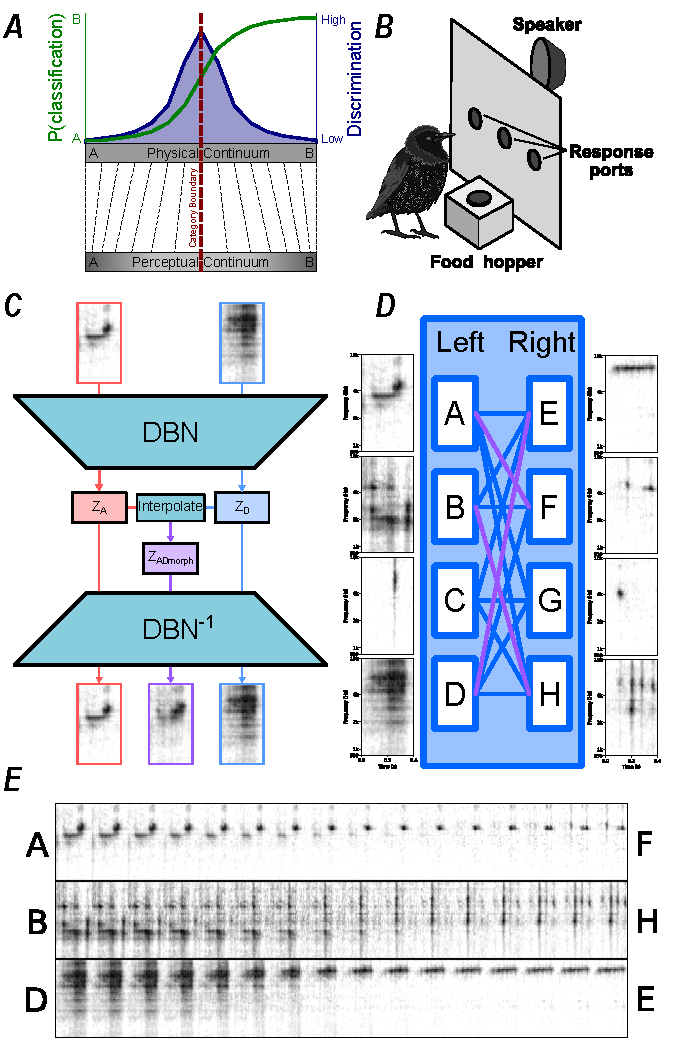
\includegraphics[width=114mm]{figures/fig01_task_outline.pdf}
  \caption[Task outline]
{(continued on following page.)
\index{outline}}
  \label{fig:outline}
\end{figure}

\begin{figure}[tp]
  \contcaption{
(A) A schematic of idealized categorical perception. \emph{Top green}: The psychometric function or the probability of classifying a stimuli as A or B as you move along a physical continuum between A and B. The category boundary occurs at the vertical red dotted line and there is some amount of uncertainty near this boundary. The boundary is defined as the point of perceived equality or the stimuli location on the physical continuum where a participant is equally likely to classify the stimuli as A or B. \emph{Top Blue}: is the discrimination curve describing how well a participant can discriminate between nearby stimuli. \CP has been described as a peak in the discrimination curve near the category boundary. The lower axis indicates how the perceptual space is stretched compared to the physical continuum causing stimuli that are within category limits to be perceived as closer than stimuli that lie across category boundaries, but are an equal distance apart.
(B) A diagram of the operant behavioral apparatus which consists of response ports with IR beak detection sensors, a food hopper to provide access to a food reward, and a speaker hidden behind the panel to present auditory stimuli.
(C) A diagram of generating an interpolating morph using a \DBN autoencoder. A spectrogram representation of two 400 ms song motif, A and D, are fed into a compressive network to create a latent representation, $Z_A$and $Z_D$. We then linearly interpolate between $Z_A$and $Z_D$ to create $Z_{ADmorph}$ which we can use to reconstruct a spectrogram motif that lies between A and D. Three example morph interpolations are shown below in (E)
(D) Diagram of the behavioral task. Spectrograms of the initial 8 randomly chosen 400 ms long motifs, labeled A-H, and their reward associated responses. Once the performance on these 8 reached a sufficient stable level, interpolated morph motifs, indicated by the 16 connecting lines were probed using a ratcheting double staircase procedure to allow the birds to determine their own behavioral boundaries.The 3 example morph dimensions displayed to the left are highlighted in blue.
(E) Three example interpolated morph dimensions generated using the \DBN. 16 (of 128 used) example motifs for each morph dimension. Spectrogram representation with frequency on y-axis and time on the x-axis. Each motif is 400 ms long.}
\end{figure}